\vspace{-2mm}
\section{{\large \bf \graphsim}}
\label{Sim}
In this section, we present \graphsim, our novel similarity computation algorithm designed for heterogeneous recommendation. 
% \graphsim is leveraged, in \crossrec, to compute the similarities between items across domains. 
%\graphsim is then used to compute the best \emph{k nearest neighbors} in the target domain.

%\vspace{-2mm}
%\subsection{Overview}
\noindent{\bf Overview.} Consider a similarity graph $G$ of which the vertices are the items and the edges are weighted by the similarities computed using the standard adjusted cosine similarity~\cite{sarwar2001item}. Typically, this metric can only identify a small number of item
similarities between different domains. Figure~\ref{fig:simCount} conveys this very fact  that we can compute around 0.3 million heterogeneous similarities\footnote{Heterogeneous similarity denotes the similarity computed between items in different domains, e.g between a book and a movie.} using this standard item-item adjusted cosine similarity (\textsc{AdCos}). Being sparse with few edges, $G$ induces very few heterogeneous connections and results in substandard recommendation quality. Clearly, this standard similarity computation is not suitable for \emph{heterogeneous} recommenders. 

In \crossrec, we use a novel meta path-based algorithm to compute an extended similarity graph. We compute the similarity between items even if they are not directly connected, and only related through some meta paths. 
Figure~\ref{fig:simCount} shows that the number of detected heterogeneous similarities is nearly an order of magnitude higher by using our meta path-based approach instead of \textsc{AdCos}. (These freshly detected heterogeneous similarities lead to better recommendation quality as we show later in \autoref{eval:accuracy}.)

%which we present precisely in this section. Roughly speaking, if two items in $G$ are not directly connected but they are associated through some paths, then we could compute the similarity between these two items based on these paths. We describe this path-based algorithm in details below.


\begin{figure}
\begin{center}
\vspace{-3mm}
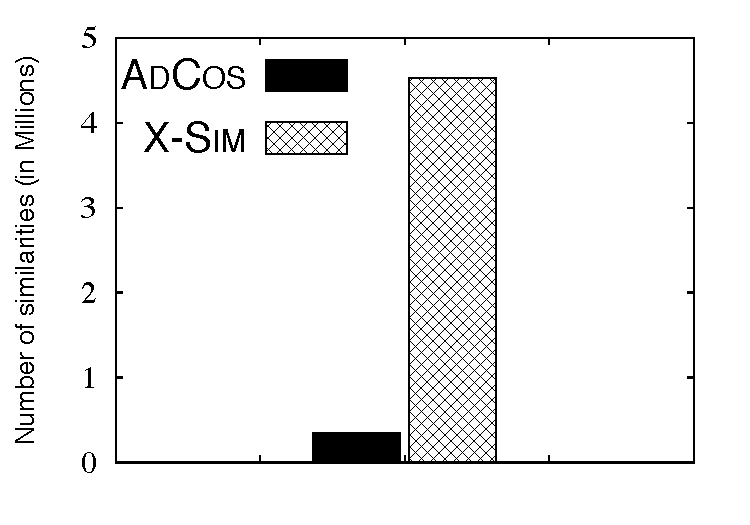
\includegraphics[height=1.6in,width=2.3in]{figures/Total_Sim.pdf}
\vspace{-6mm}
\caption{{\bf The number (millions) of inter-item similarities computed for the Amazon dataset using adjusted cosine similarity and \graphsim.}}
\label{fig:simCount}
\end{center}
\end{figure}

%\vspace{-2mm}
%\subsection{Baseline Similarity Graph}
\noindent{\bf Baseline Similarity Graph.} Our first step is to build the baseline similarity graph. There are several known methods for computing item-item similarities, e.g. Cosine, Pearson, Adjusted-cosine~\cite{sarwar2001item}. Though \graphsim can support any similarity metric as its baseline, we use adjusted-cosine which is shown to be more effective than the others~\cite{sarwar2001item}:
\begin{equation}
s_{ac}(i,j)=\frac{\sum _{u \in Y_i \cap Y_j} (r_{u,i} - \bar{r_u})(r_{u,j} - \bar{r_u})}{\sqrt{\sum _{u \in Y_i} (r_{u,i} - \bar{r_u})^2}\sqrt{\sum _{u \in Y_j} (r_{u,j} - \bar{r_u})^2}}
\label{adcos}
\end{equation}
In this first step, we compute the (baseline) similarities by integrating both $S$ and $T$ as a single domain. We denote by $G_{ac}$ the resulting similarity graph.\footnote{Here \emph{ac} denotes adjusted cosine.} We address the sparsity issue of $G_{ac}$ (Figure~\ref{fig:simCount}) by considering meta paths connecting both domains and then by extending $G_{a c}$. Clearly, a brute-force scheme considering all possible paths would be inefficient and not scalable. Assuming $m$ items in the database, the time complexity of such a brute-force scheme (computing path similarity for every pair of items) is $O(m^2)$, which is not suitable for big datasets like the Amazon one. \crossrec uses a layer-based pruning technique to consider only $O(k)$ paths for each item where $k \lll  m$. This pruning technique reduces the time complexity to $O(km) \simeq O(m)$.


\begin{figure}
\begin{center}
\includegraphics[height=1.8in,width=3.2in]{figures/dom_Cat.png}
\vspace{-2mm}
\caption{{\bf The layer-based pruning technique used in \crossrec.}}
\label{fig:domcat}
\end{center}
\end{figure}

%\vspace{-2mm}
%\subsection{X-Sim}
\noindent{\bf Layer-based Pruning.} Based on the baseline similarity graph, any item $i$ in a domain $D$ which connects to some item $j$ in another domain $D'$ is called a \emph{bridge item}. Both $i$ and $j$ are bridge items in this case. Any item that is not a bridge item is called a \emph{non-bridge item}. 

\crossrec's pruning technique partitions the items from $S$ and $T$ into six layers, as depicted in Figure~\ref{fig:domcat}. In turn, the items in each domain, say $D$, are divided into three layers (Figure~\ref{fig:domcat}).

\begin{itemize}
\item {\it BB-layer.} The (Bridge, Bridge)-layer consists of the bridge items of $D$ connected to the bridge items of another domain.

\item {\it NB-layer.} The (Non-bridge, Bridge)-layer consists of the non-bridge items of $D$ which are connected to bridge items of $D$.

\item {\it NN-layer.} The (Non-bridge, Non-bridge)-layer consists of the non-bridge items of $D$ which are not connected to other bridge items.
\end{itemize}

\crossrec then considers only the paths crossing different layers denoted by \emph{meta paths}.  Since a $k$-nearest neighbor method is used for the recommendation, \crossrec chooses, for each item $i$, the top-$k$ items from every neighboring layer. Let $G$ be the resulting top-$k$ similarity graph, which \crossrec treats as an undirected graph, i.e. if $i$ is one of $j$'s top-$k$ neighbors or $j$ is one of $i$'s top-$k$ neighbors then $i$ and $j$ are connected in $G$. Each node in $G$ has thus a degree at most $2k$. We describe the meta path selection via layers in more details in~\autoref{Implementation}.


\noindent{\bf \graphsim.} Consider any two items $i$ and $j$. We denote by $Y_{i \geq \bar{i}}$ the set of users who rated item $i$ higher than or equal to the average rating for $i$ over all the users in the database who rated it. We also denote by $Y_{i < \bar{i}}$ as the set of users who rated item $i$ lower than the average rating for $i$. Additionally, we denote by $n(Y_i)$ the cardinality of the set $Y_i$. 

\begin{definition}[Weighted Significance]
Given a pair of items $i$ and $j$, we define weighted significance ($S_{i,j}$) as the number of users who mutually agree or disagree on their preference for this pair. More precisely, we define the weighted significance ($S_{i,j}$) between $i$ and $j$ as follows.
$$
S_{i,j}= \underbrace{\left\vert{Y_{i \geq \bar{i}} \cap Y_{j \geq \bar{j}}}\right\vert}_\text{Mutual agreement} + \underbrace{\left\vert{Y_{i < \bar{i}} \cap Y_{j < \bar{j}}}\right\vert}_\text{Mutual disagreement}
$$
%$$
%S_{i,j}= \underbrace{n(Y_{i \geq \bar{i}} \cap Y_{j \geq \bar{j}})}_\text{Mutual agreement} + \underbrace{n(Y_{i < \bar{i}} \cap Y_{j < \bar{j}})}_\text{Mutual disagreement}
%$$
\end{definition}
Intuitively, higher significance value implies higher importance of the similarity value. For example, a similarity value of 0.5 between an item-pair ($i$,$j$) with $S_{i,j}=1000$ is more significant than a similarity value of 0.5 between an item-pair ($i$,$k$) with $S_{i,k}=1$ (for the latter may be a result of pure coincidence).

\begin{definition}[Meta Path]
Given $G$ and its six corresponding layers of items, we define a meta path as the path that contains at most one item from each layer.
\end{definition}
For every meta path $p = i_1 \leftrightarrow i_2 \ldots \leftrightarrow i_k$, we compute the path similarity $s_p$, weighted by its significance value, as follows.
\[ s_p = \frac{\sum_{t=1}^{t=k-1} S_{i_{t},i_{t+1}} \cdot s_{a c} (i_{t}, i_{t+1})}{\sum_{t=1}^{t=k-1}  S_{i_{t},i_{t+1}}}  \]
%\[ s_p = \frac{S_{i_1,i_2} \cdot s_{a c} (i_1, i_2) + \ldots + S_{i_{k-1},i_k} \cdot s_{a c} (i_{k - 1}, i_k)}{S_{i_1,i_2} + \ldots + S_{i_{k-1},i_k}} \]

For each pair of items $(i, j)$ from different domains, if $i$, $j$ are not connected directly, we aggregate the path similarities of all meta paths connecting $i$ and $j$. Due to the different lengths and similarities for paths, we have to give different weights to different paths. Shorter paths produce better similarities in recommenders~\cite{ramakrishnan2001privacy,sun2011pathsim} and hence are more preferred over longer ones. We now explain the strategy behind assigning these weights and thereby computing the \graphsim values.

\begin{definition}[Fractional Weighted Significance]
Given a pair of items $i$ and $j$, we define fractional weighted significance ($F_{i,j}$) between $i$ and $j$ as their significance value weighted by the inverse of number of users rating either $i$ or $j$. More precisely, we denote fractional weighted significance as follows. $$
F_{i,j}=\frac{S_{i,j}}{n(Y_i \cup Y_j)}
$$
\end{definition}

%We denote \emph{fractional mutuality} ($F_{i,j}$) between $i$ and $j$ as:

Next, we define the notion of \emph{path certainty} ($c_p$) of a meta path to take into account the factor of varying path lengths.
\begin{definition}[Path Certainty]
Given a meta path ($p = i_1 \leftrightarrow i_2 \ldots \leftrightarrow i_k$), we compute the path certainty ($c_p$) of the meta path $p$ as the product of the fractional weighted significance between each consecutive pair of items in the path $p$. More precisely, we define the path certainty as follows.
$$
c_p= \prod_{t=1}^{t=k-1} F_{i_{t}, i_{t+1}}
$$
%$$
%c_p= F_{i_1,i_2} \times \ldots \times F_{i_{k-1},i_k}
%$$ 
\end{definition}

Finally, we define our \graphsim metric as follows.

\begin{definition}[X-Sim]
Let $P (i, j)$ denote the set of all meta paths connecting items $i$ and $j$. We define the \graphsim for the item pair (i,j) as the path similarity weighted by the path certainty for all paths in $P(i,j)$. More precisely, we define \graphsim for any given pair of items $i$ and $j$ as follows.
$$
\textsc{X-Sim} (i, j) = \frac{\underset{p \in P (i, j)}{\sum} c_p \cdot s_p}{\underset{p
   \in P (i, j)}{\sum} c_p} 
$$
\end{definition}


%RGRG shouldn't this be a footnote?
Here, \graphsim{($i$,$j$)} denotes the heterogeneous similarity between any two items $i$ and $j$. Note that a trivial transitive closure over similarities would not take into account these factors, which would in turn impact the heterogeneous similarities and the recommendation quality.
